\section{Evaluation}\label{sec:eval}

We evaluated the Omni coarray compiler on the systems shown in \tab{specs}.

\begin{table}
 \begin{center}
  \caption{Specs of the compulters used for evaluation}\label{tab:specs}
  \begin{tabular}{l|p{0.4\textwidth}|p{0.4\textwidth}}
   \hline
   & HOKUSAI GreatWare (RIKEN RCCS)   & CCS, University of Tsukuba \\
   & Fujitsu PRIMEHPC FX100           & HA-PACS/TCA \\
   \hline
   \hline
   CPU
   & SPARK64\texttrademark XIfx, 1.975GHz, 1CPU per node, 4-SIMD $\times$ 32-core
   & E5-2680 v2 (Ivy Bridge), 10-core, 224GFlops, 2CPU per node \\
   \hline
   memory
   & 32GB per node, bandwidth 480GB/s per node
   & DDR3 SDRAM 128GB per node, 119.4GB/s   \\
   \hline
   interconnect
   & Tofu2, 12.5GB/s $\times$ 2
   & InfiniBand FDR, 7GB/s \\
   \hline
   compiler
   & Fujitsu Fortran Ver.\ 2.0.0 P-id:T01776-01
   & Intel Fortran 16.0.4 \\
   \hline
   MPI
   & Fujitu MPI Ver.\ 2.0.0 P-id:T01776-01 (OpenMPI base)
   & Intel MPI 5.1.3 \\
   \hline
   comm.\ layer
   & Tofu library
   & GASNet 1.24.2 built as IBV-conduit with Intel compilers \\
   \hline
  \end{tabular}
 \end{center}
\end{table}



%-----------------------------------------------------------------------------
\subsection{Fundamental Performance}
%-----------------------------------------------------------------------------

%===============
% 説明
%===============

Using EPCC Fortran Coarray micro-benchmark~\cite{EPCC}, we evaluated ping-pong performance 
of PUT and GET communications compared with MPI\_Send/Recv.
The codes are shortly shown in \tab{pingpong-code}.

%-- pingpong-code.pdf
\begin{table}[bht]
  \begin{center}
    \caption{pingpong-code.pdf}\label{tab:pingpong-code}
    % trimはleft bottom right topの順
    \mbox{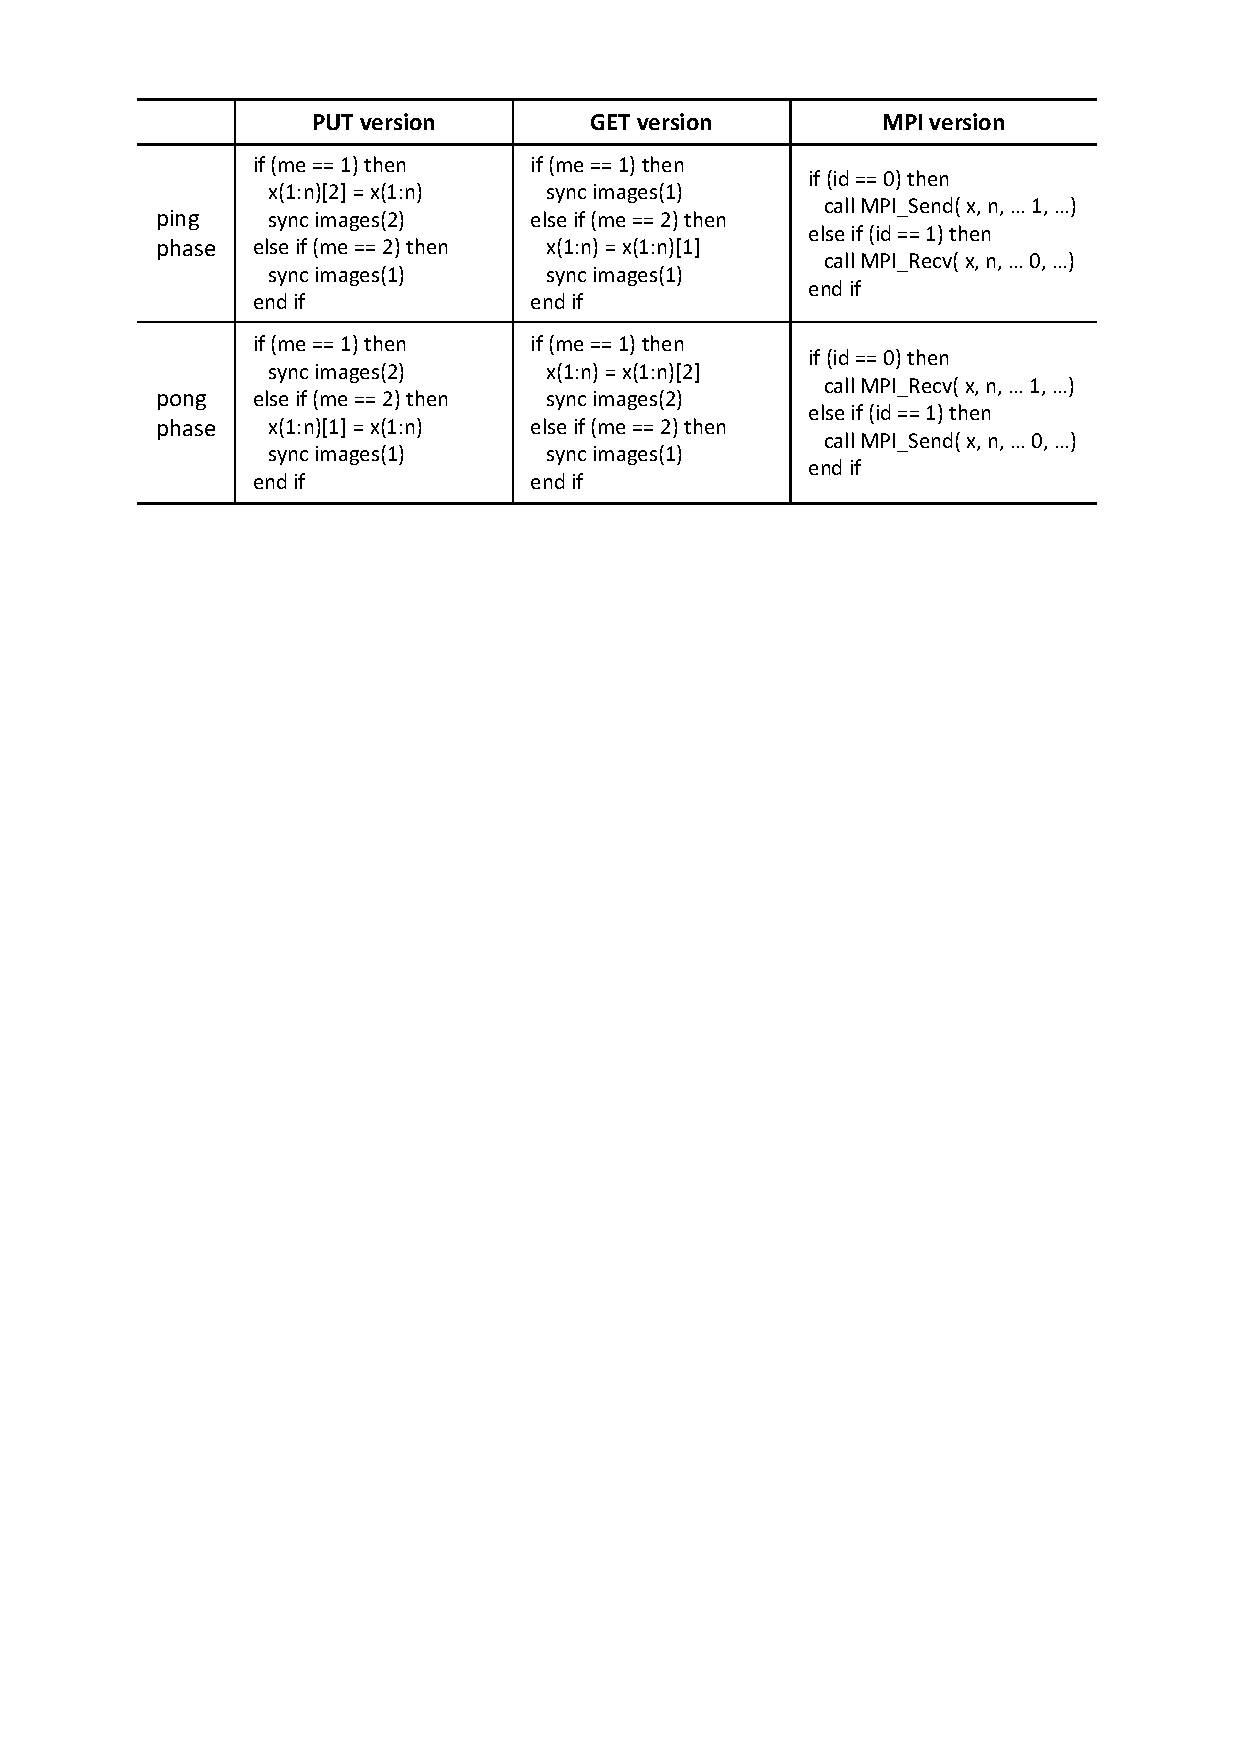
\includegraphics[trim=24mm 211mm 24mm 16mm, scale=0.7,clip]{figs/pingpong-code-r2.pdf}}
    \begin{flushright}
      {\tt me} is the image index. {\tt id} is the MPI rank number.
    \end{flushright}
  \end{center}
\end{table}

%-- pingpong-fig.pdf
\begin{figure}[bht]
  \begin{center}
    \mbox{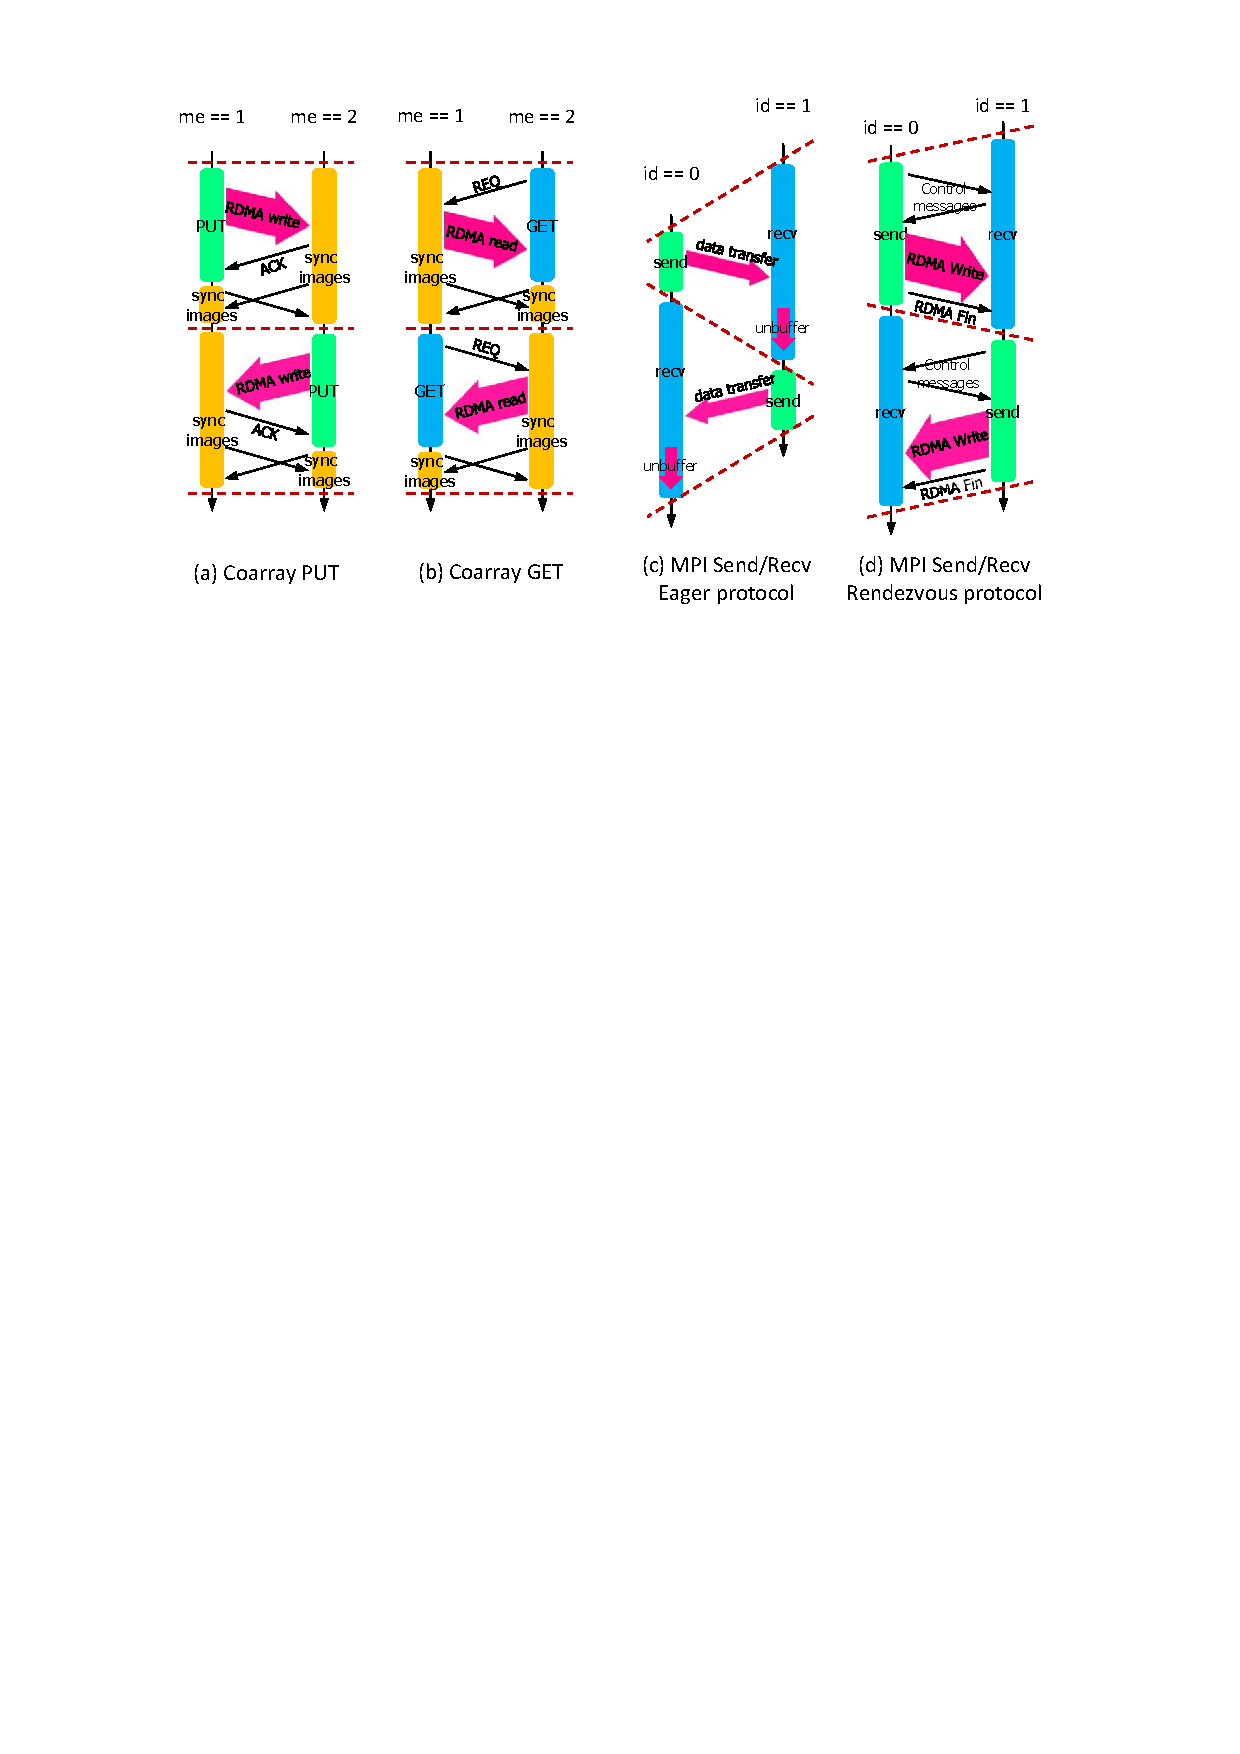
\includegraphics[trim=30mm 195mm 32mm 16mm, scale=0.75,clip]{figs/pingpong-fig-r2.pdf}}
    \caption{pingpong-fig.pdf}\label{fig:pingpong-fig}
  \end{center}
\end{figure}

Corresponding to the codes in \tab{pingpong-code}, \fig{pingpong-fig} shows how data and 
messages are echanged between two images or processes.
In coarray PUT (a) and GET (b), inter-image synchronization is necessary for each end of 
phases to make the passive image active and to make the active image passive.
While, in MPI message-passing (c) and (d), such synchronization is not necessary because
both processes are always active.
%
On the other hand, MPI message-passing has its own overhead that coarray PUT/GET
does not have. Because the eager protocol (c) does not use RDMA, the receiver
must copy the received data in the local buffer to the target. The larger the data,
the greater the overhead cost.
In the rendezvous protocol (d), negotiations including remote address notification
are required prior to the communication.
The overhead cost is not negligible when the data is small.


%===============
% 結果
%===============

\begin{figure}
  \begin{center}
    % trimはleft bottom right topの順
    \mbox{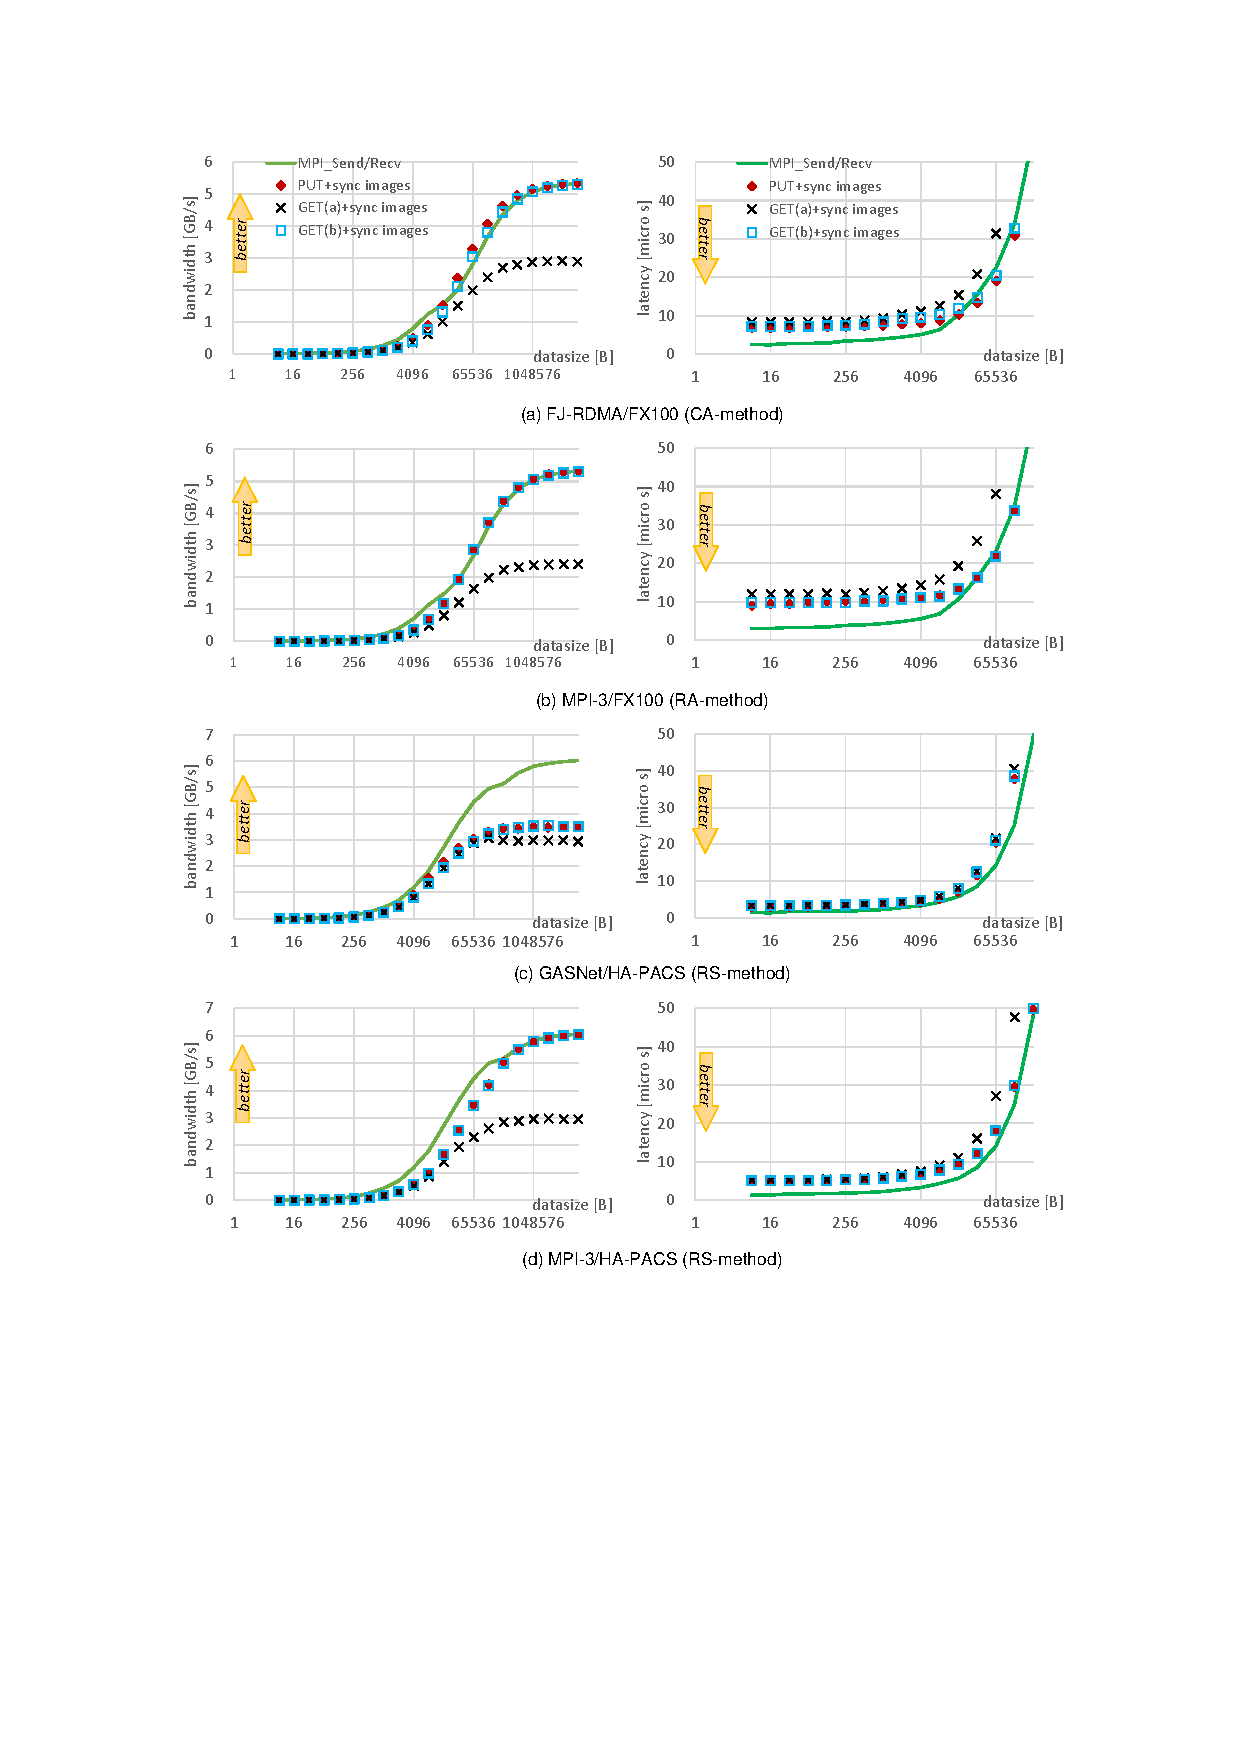
\includegraphics[trim=30mm 80mm 30mm 25mm, scale=0.8, clip]{graphs/8graphs-7.pdf}}
    \caption{Ping-pong performance on Fujitsu PRIMEHPC FX100 and HA-PACS/TCA}\label{fig:8graphs}
  \end{center}
\end{figure}

The result of the comparision between coarray PUT/GET and MPI message passing is shown in
\fig{8graphs}.
As the underlying communication libraries, 
FJ-RDMA and MPI-3 are used on FX100 and GASNet and MPI-3 are used on HA-PACS.
GET(a) and GET(b) are using the code without and with the optimization described in
\Sec{opt-get}, respectively.
Bandwidth is the communication data size per elapsed time, and
latency is half of the ping-pong elapsed time.
The difference between GET(a) and (b) is the compile-time optimization level of the 
coarray translator described in \Sec{opt-get}.

%===============
% 分かったこと
%===============

As the result, the following was found about coarray PUT/GET communication.

\begin{enumerate}

\item {\em Bandwidth.}
Coarray PUT and GET are slightly outperforms MPI rendezvous communication for large data 
on FJ-RDMA and MPI-3.
On FJ-RDMA/FX100 (a), the bandwidth of PUT and GET(b) are respectively 
+0.1\% to +18\% and -0.4\% to +9.3\% higher than MPI rendezbous in the 
rendezvous range of 32k through 32M bytes.
Also on MPI-3/HA-PACS, respectively +0.3\% to +0.8\% and 
+0.1\% to +1.3\% higher in the rendezvous range of 512k through 32M bytes.

It was confirmed from the runtime log that zero-copy communication was performed
both in PUT and GET(b) by selecting DMA scheme described in \Sec{opt-dma}.

However, on GASNet/HA-PACS (c), PUT and GET(b) has only about 60\% bandwidth for large data
than MPI rendezvous.
It is presumed that data copy was caused internally.

\item {\em Latency.}
On FJ-RDMA (a) and MPI-3 (b) and (d), PUT and GET(b) have larger (worse) latency than 
MPI eager communication, in the range of $\leq$16kB on FX100 and $\leq$256kB on HA-PACS.

Coarray on GASNet (c) behaves differently than other cases on (a), (b) and (d).
Though the latency is larger than the one of MPI for all data sizes, the difference
is smaller than the other cases. At data size 8B, the latency of PUT is 2.93$\mu$s
and 2.1 times larger than the one of MPI 
while 5.73$\mu$s and 3.7 times larger on the case of MPI-3 (d).

\item {\em Effect of GET optimization.}
For all ranges of all cases, GET(a) has smaller bandwidth and larger latency than GET(b).
On FJ-RDMA (a), the bandwidth is 1.41 to 1.85 times improved in the range of 32kB to 32MB
by changing the object code of GET(a) to (b).
We found GET(a) caused two extra memory copies; one is performing the array assignment 
by the Fortran library and the other is the copy from the communication buffer 
to the result variable of the array function {\tt xmpf\_coarray\_get\_generic}. 
The optimization described in \Sec{opt-get} has eliminated these two data copies.

\end{enumerate}

The issue is the large latency of coarray PUT/GET communication.
In the next subsection, it is discussed how it should be solved 
by the compiler and the programming.



%===========================================================
\subsection{Non-blocking communication}
%===========================================================

For latency hiding, asynchronous and non-blocking features can be expected 
on coarray PUT communication.
The principle is shown in \fig{nonblock-fig}.
%
\fig{nonblock-fig} (a) illustrates the half pattern of the ping-pong PUT communication.
Coarray one-sided communication is basically asynchronous unless 
synchronization is explicitly specified. Therefore, multiple communications
without synchronization between them, as shown in (b), is closer to actural applications.
In addition, it can be optimized using non-blocking communication as shown in (c).
Blocking and non-blocking communications can be switched with the runtime environment
variable in the current implementation of the Omni compiler.
In MPI message passing, non-blocking communication can be written with 
{\tt MPI\_Isend}, {\tt MPI\_Irecv} and {\tt MPI\_Wait}.

%-- nonblock-fig.pdf
\begin{figure}[tbh]
  \begin{center}
  % trimはleft bottom right topの順
    \mbox{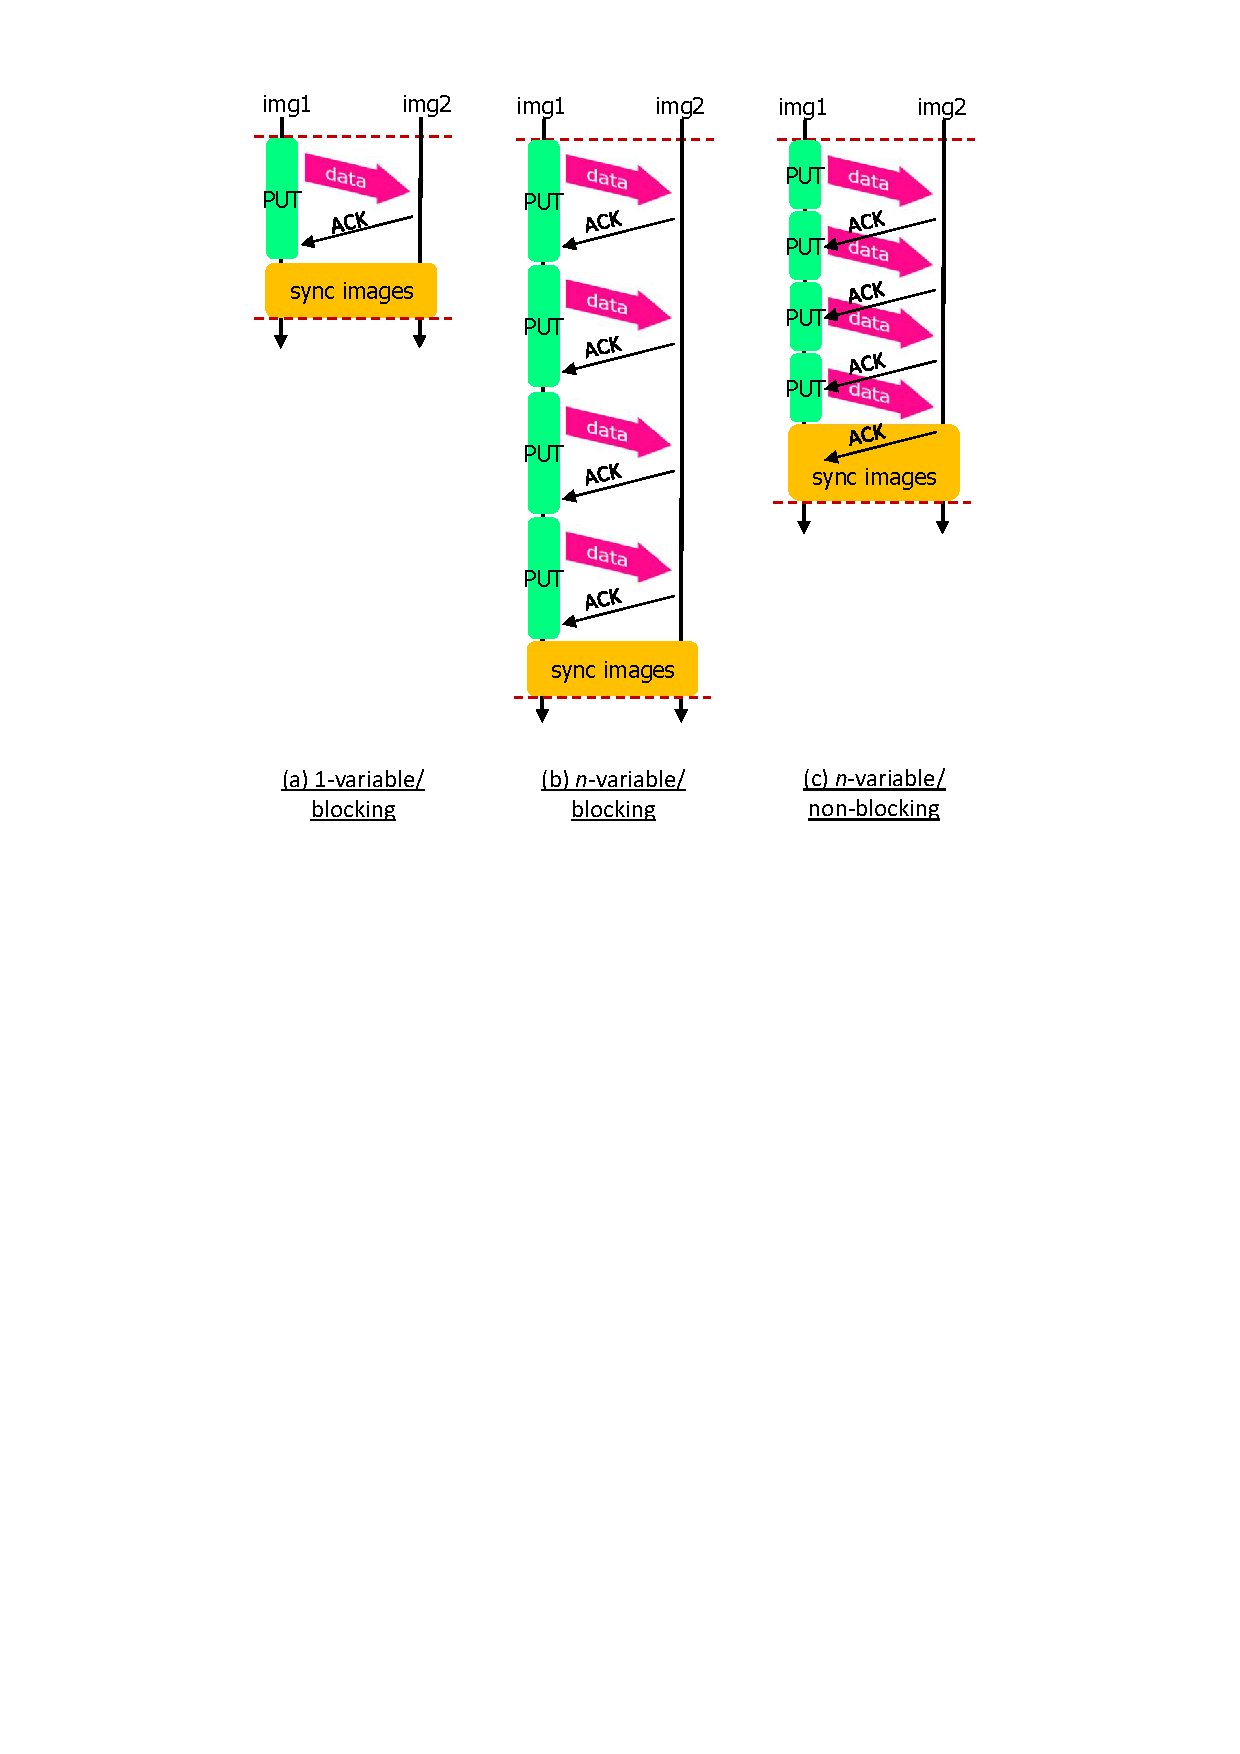
\includegraphics[trim=43mm 144mm 43mm 3mm, scale=0.6,clip]{figs/nonblock-fig-r2.pdf}}
    \caption{nonblock-fig.pdf}\label{fig:nonblock-fig}
  \end{center}
\end{figure}


\fig{8var-pingpong} shows the result of 8-variable ping-pong, which repeats
that sending eight separate pieces of data from one to the other in order 
and then doing similarly in the opposite direction.
Since each blocksize indicates the size of the piece, 

In non-blocking communications PUT non-blocking and {\tt MPI\_Isend/Irecv},


(2) Non-blocking communication. Since the CAF language specification does 
not guarantee the arrival order of the PUT communications unless they are 
partitioned by explicit synchronization, it is possible to continue multiple 
non-blocking communication until the synchronization is encountered. The access 
order on the local side is guaranteed by the Omni runtime using the buffering 
method rather than the DMA. The expected execution of n-variable non-blocking 
PUT is illustrated in Figure 6(c). FJ-RDMA has a function that counts the 
number of unconsumed ACK signals, which is required on multiple non-blocking 
communication. The code is the same as the one for blocking communication 
shown in (c) of Table 3 and the runtime is modified so that it can be switched 
by the environment variable. For comparative evaluation, the MPI code is modified 
to Table 3(b).

Figure 7 compares the results of n-variable blocking/non-blocking MPI two-sided 
communications ({\tt MPI\_Send/Recv} and {\tt MPI\_Isend/Irecv}) and CAF PUT 
communications (hereinafter referred to as MPI blocking, MPI non-blocking, 
PUT blocking and PUT non-blocking, respectively). On the K computer, it is 
shown that the latency of PUT non-blocking decreases as the number of variable 
increases and it is the lowest of the four on 8-variable for 128 bytes or more. 

Meanwhile, MPI non-blocking has little effect on improving latency from MPI 
blocking and it is somewhat worse on 1- and 2-variable ping-pong. The effect 
of non-blocking is obviously greater for CAF PUT than for MPI two-sided. On 
PRIMEHPC FX100, a similar tendency was seen and the latency of PUT non-blocking 
was the lowest for 8-variable ping-pong when the block size is 32 bytes or more.

The advantage of multi-variable non-blocking communication is clarified by 
the bandwidth measurement. Figure 8 compares the bandwidth of the four for 
8-variable. The following tendencies can be found in the graph:

1.The peak bandwidths of MPI blocking and PUT blocking are almost the same, 
and the difference is at most 1\% when the block size is 2MB or more.

2.The peak bandwidth of MPI non-blocking and PUT non-blocking are almost the 
same, and the difference is at most 1\% when the block size is 256kB or more.

3.MPI non-blocking has higher bandwidth than MPI blocking when the block size 
is large. The maximum 2.0 times difference occurs when the block size is 64kB, and rendezvous communication seems to start from there.

4.PUT non-blocking has higher bandwidth than MPI blocking when the block size 
is medium. It is the maximum 2.6 times faster when the block size is 8kB and 
more than 20\% faster when the block size is 8B to 32kB

Item 1 and 2 mean that the same amount of works that are not covered with 
the latency is hiding both in non-blocking MPI and in non-blocking PUT. Taking 
item 4 into account, more work was left uncovered with the latency hiding 
in non-blocking MPI compared to non-blocking PUT. We think the extra work 
in MPI contains 1) communication to tell the target global address on the 
receiver to the sender in the case of the rendezvous method, and 2) memory 
copy from the buffer to the target data on the receiver in the case of the 
eager method. In contrast, in non-blocking PUT, 1) the communication for the 
target address is not needed because the base address has been registered 
previously and the offset is described in the code of the sender side, and 
2) RDMA is always used in the Omni CAF runtime. 

Based on the results described in this subsection, we found a condition under 
which coarray PUT communication outperforms MPI two-sided communication. When 
the communication data fragments are shorter than ~1MB, they should be aggregated 
between explicit synchronizations by the programmer and be performed in non-blocking 
by the runtime library. A practical example is shown in the next subsection.




\begin{figure}
  \begin{center}
    %-- 8var-pipo-latency.pdf
    \fbox{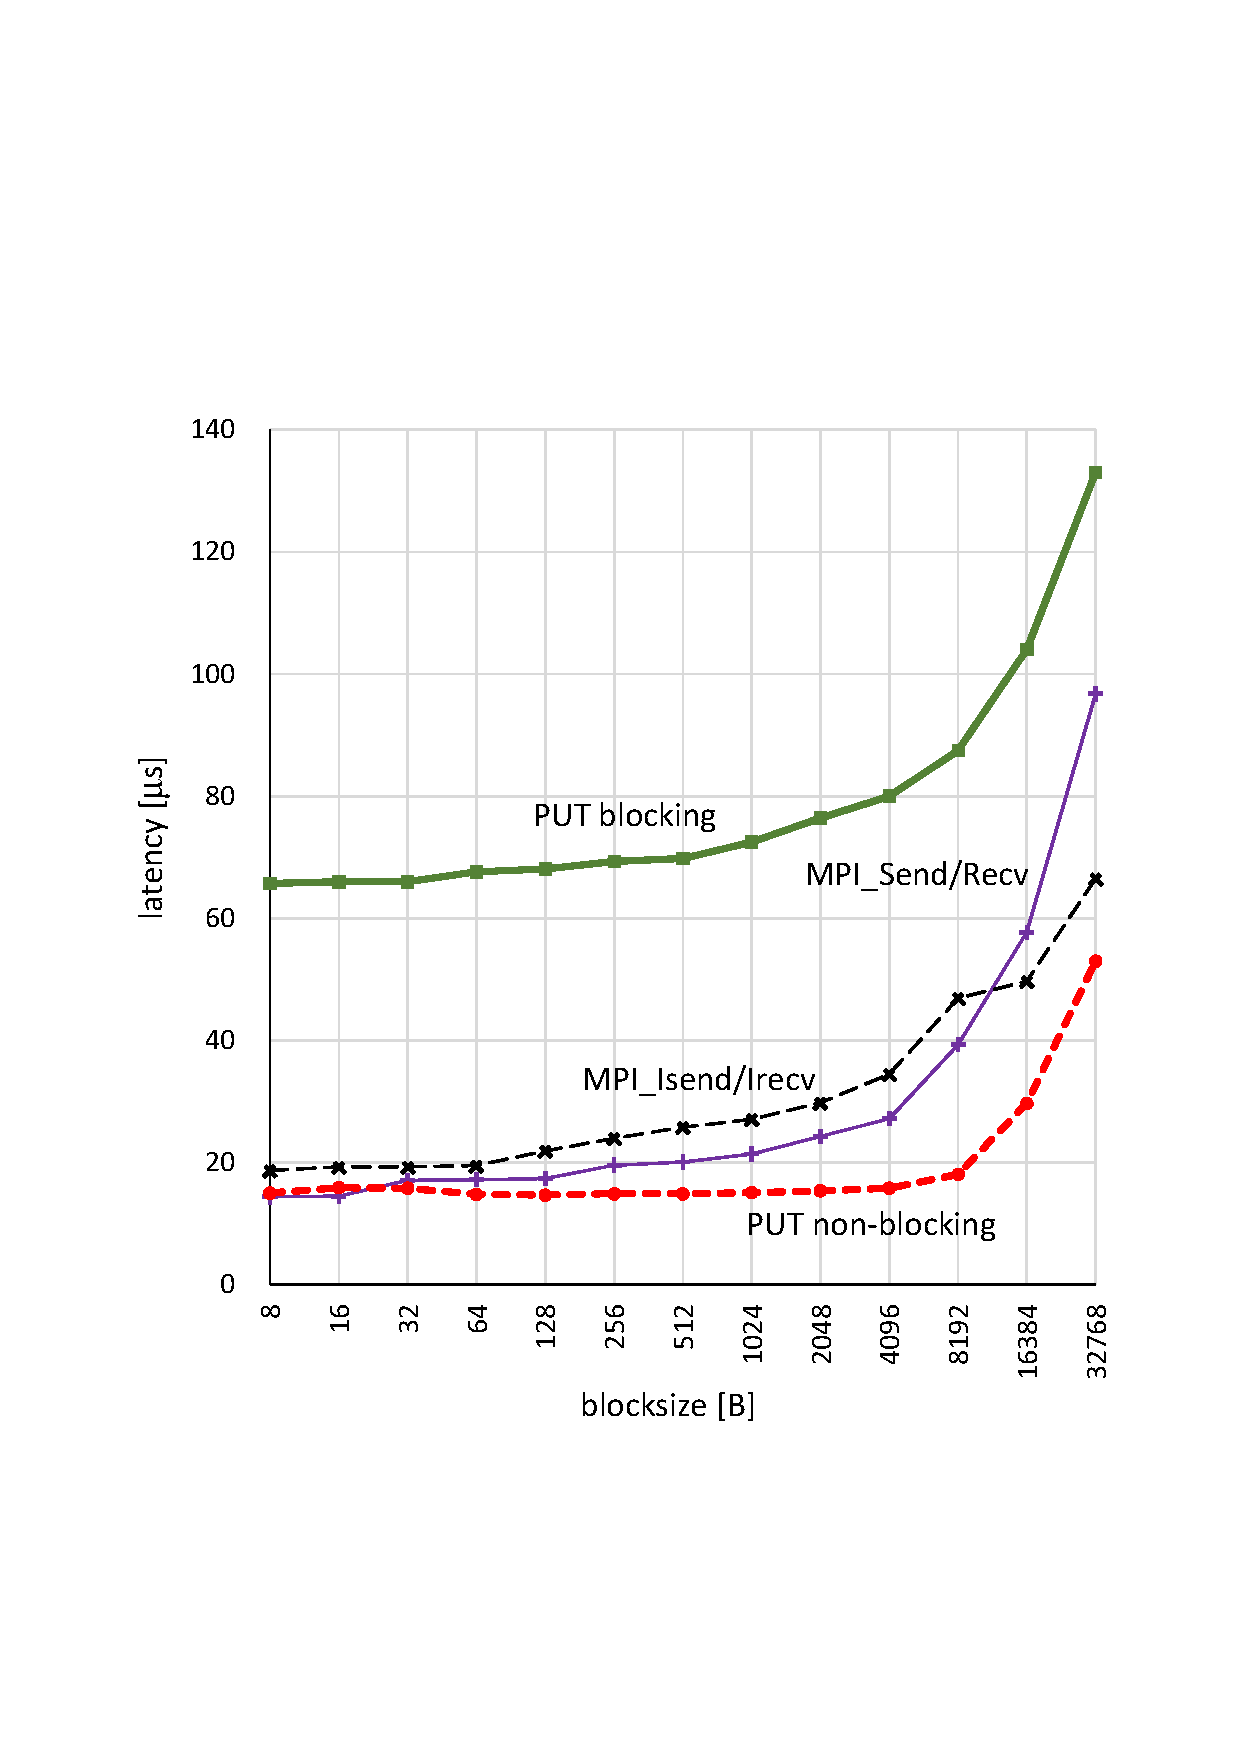
\includegraphics[trim=15mm 50mm 5mm 50mm, scale=0.6, clip]{graphs/8var-latency.pdf}}
    \caption{8-variable ping-pong latency on PRIMEHPC FX100}\label{fig:8var-pingpong}
   \end{center}
\end{figure}
    

%\begin{figure}
%  \begin{center}
%    %-- 8var-pipo-bw.pdf
%    \mbox{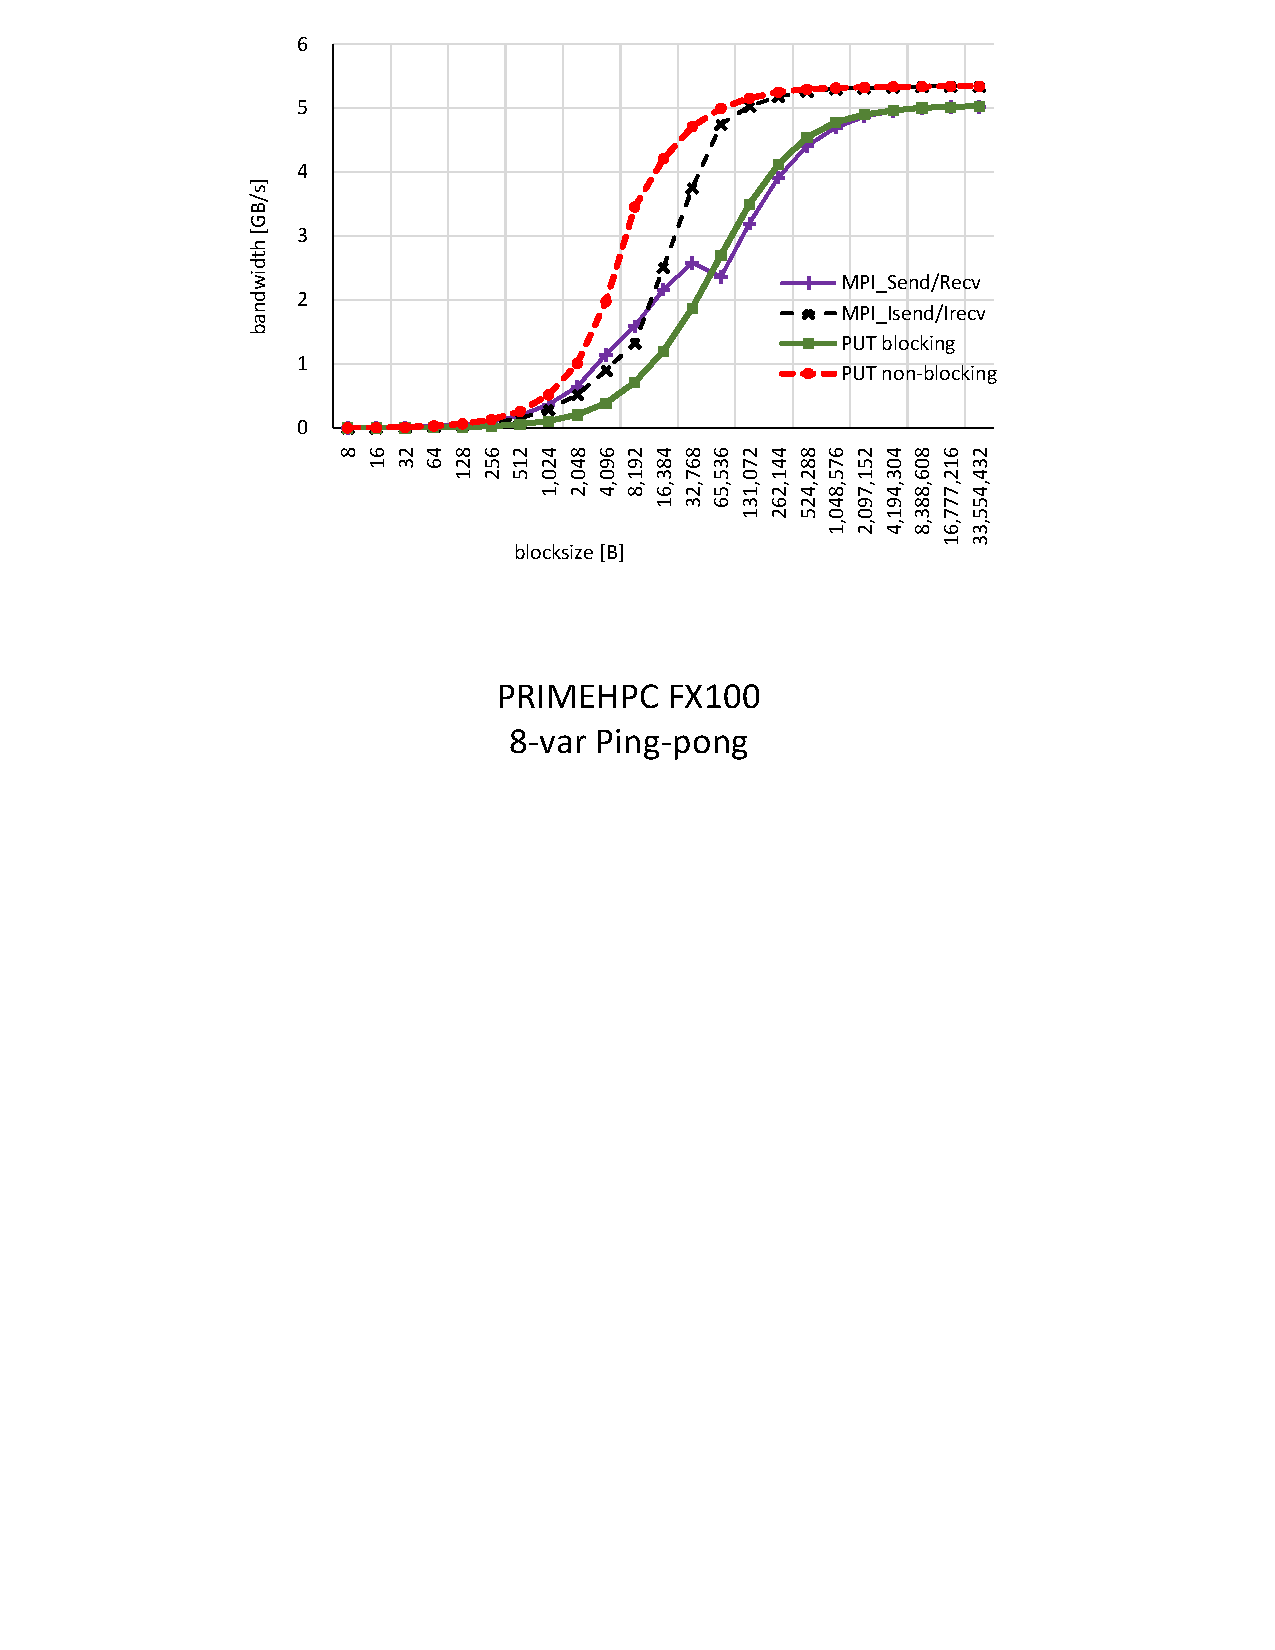
\includegraphics[trim=40mm 180mm 43mm 0mm, scale=0.6,clip]{figs/8var-pipo-bw.pdf}}\\
%    (a) Bandwidth of blocking and non-blocking communications\\
%    %-- 8var-pipo-latency.pdf
%    \mbox{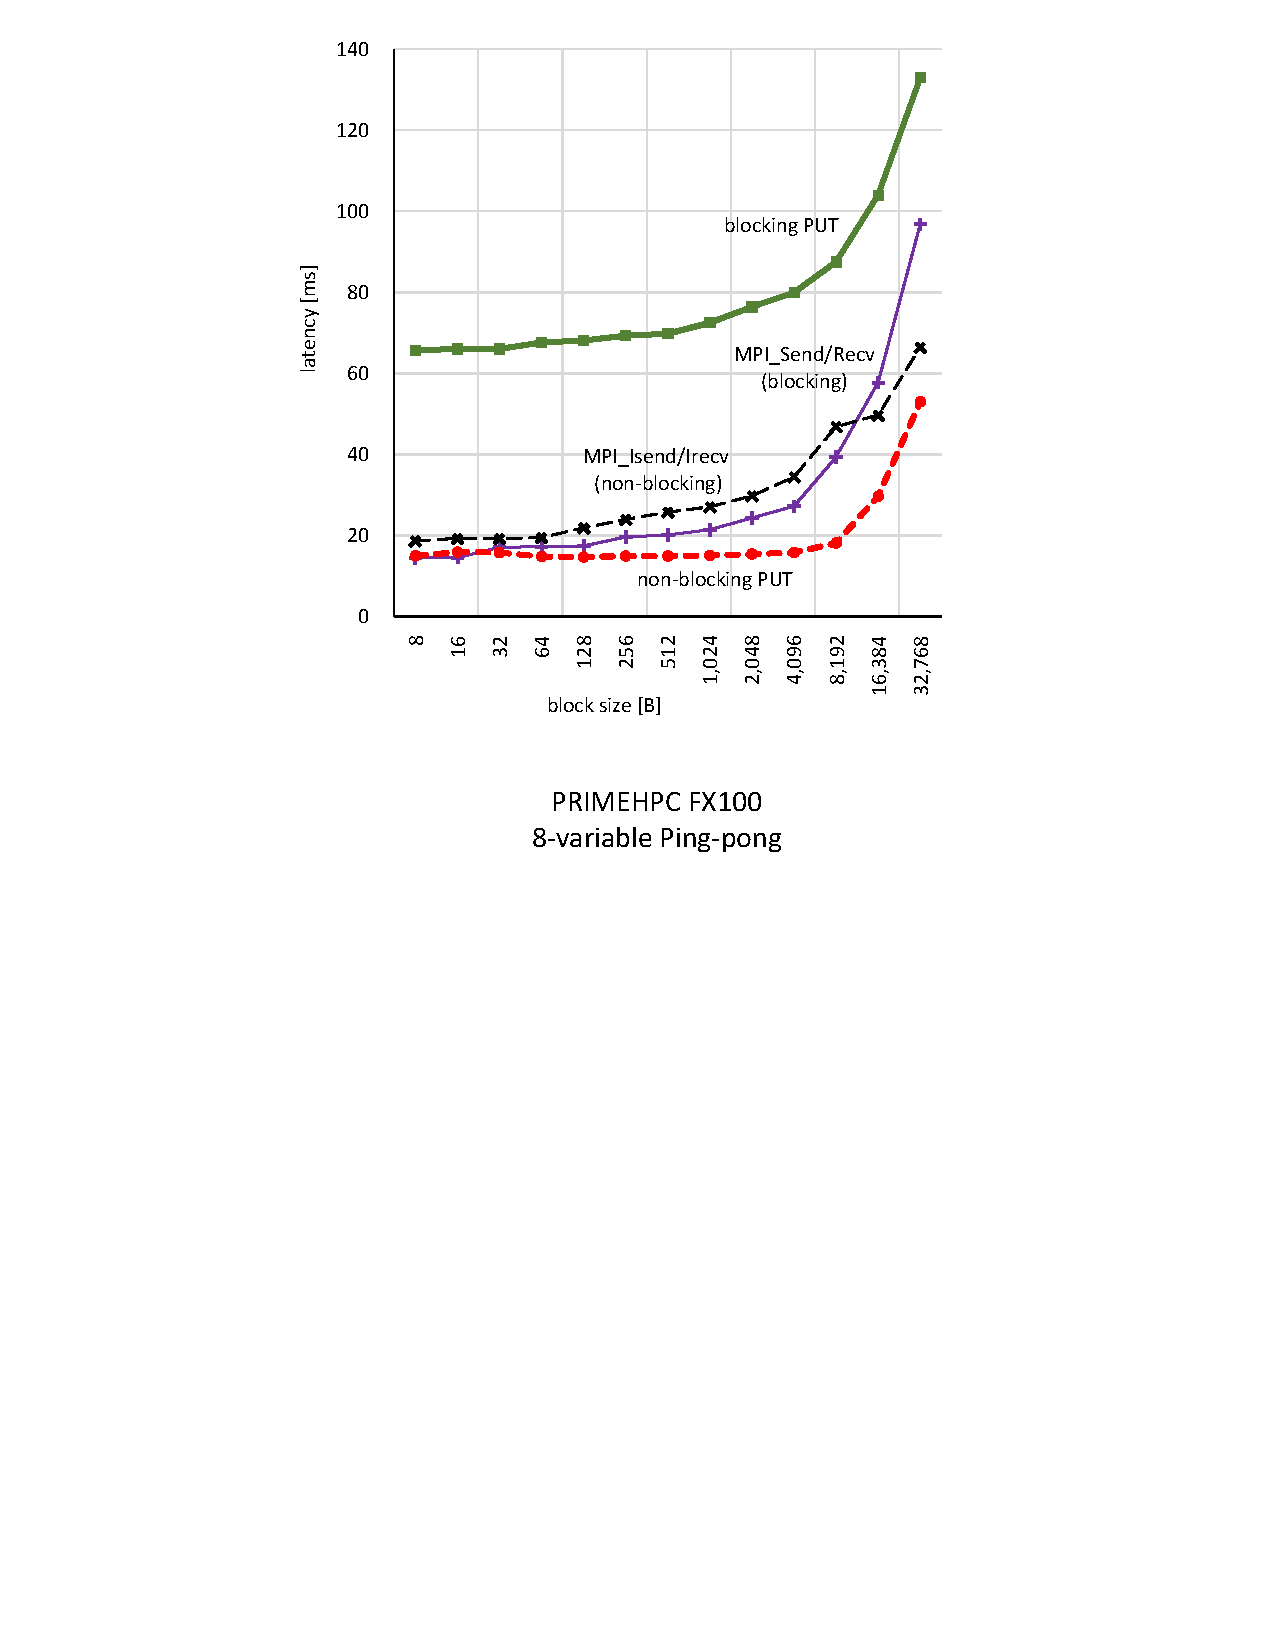
\includegraphics[trim=40mm 155mm 40mm 0mm, scale=0.6,clip]{figs/8var-pipo-latency.pdf}}\\
%    (b) Latency of blocking and non-blocking communications
%    \caption{8-variable ping-pong on PRIMEHPC FX100}\label{fig:8var-pingpong}
%   \end{center}
%\end{figure}






\subsection{Himeno Benchmark}

説明はどこかにある。\fig{himeno-graph}

%-- himeno-graph.pdf
\begin{figure}[p]
  \begin{center}
  % trimはleft bottom right topの順
    \mbox{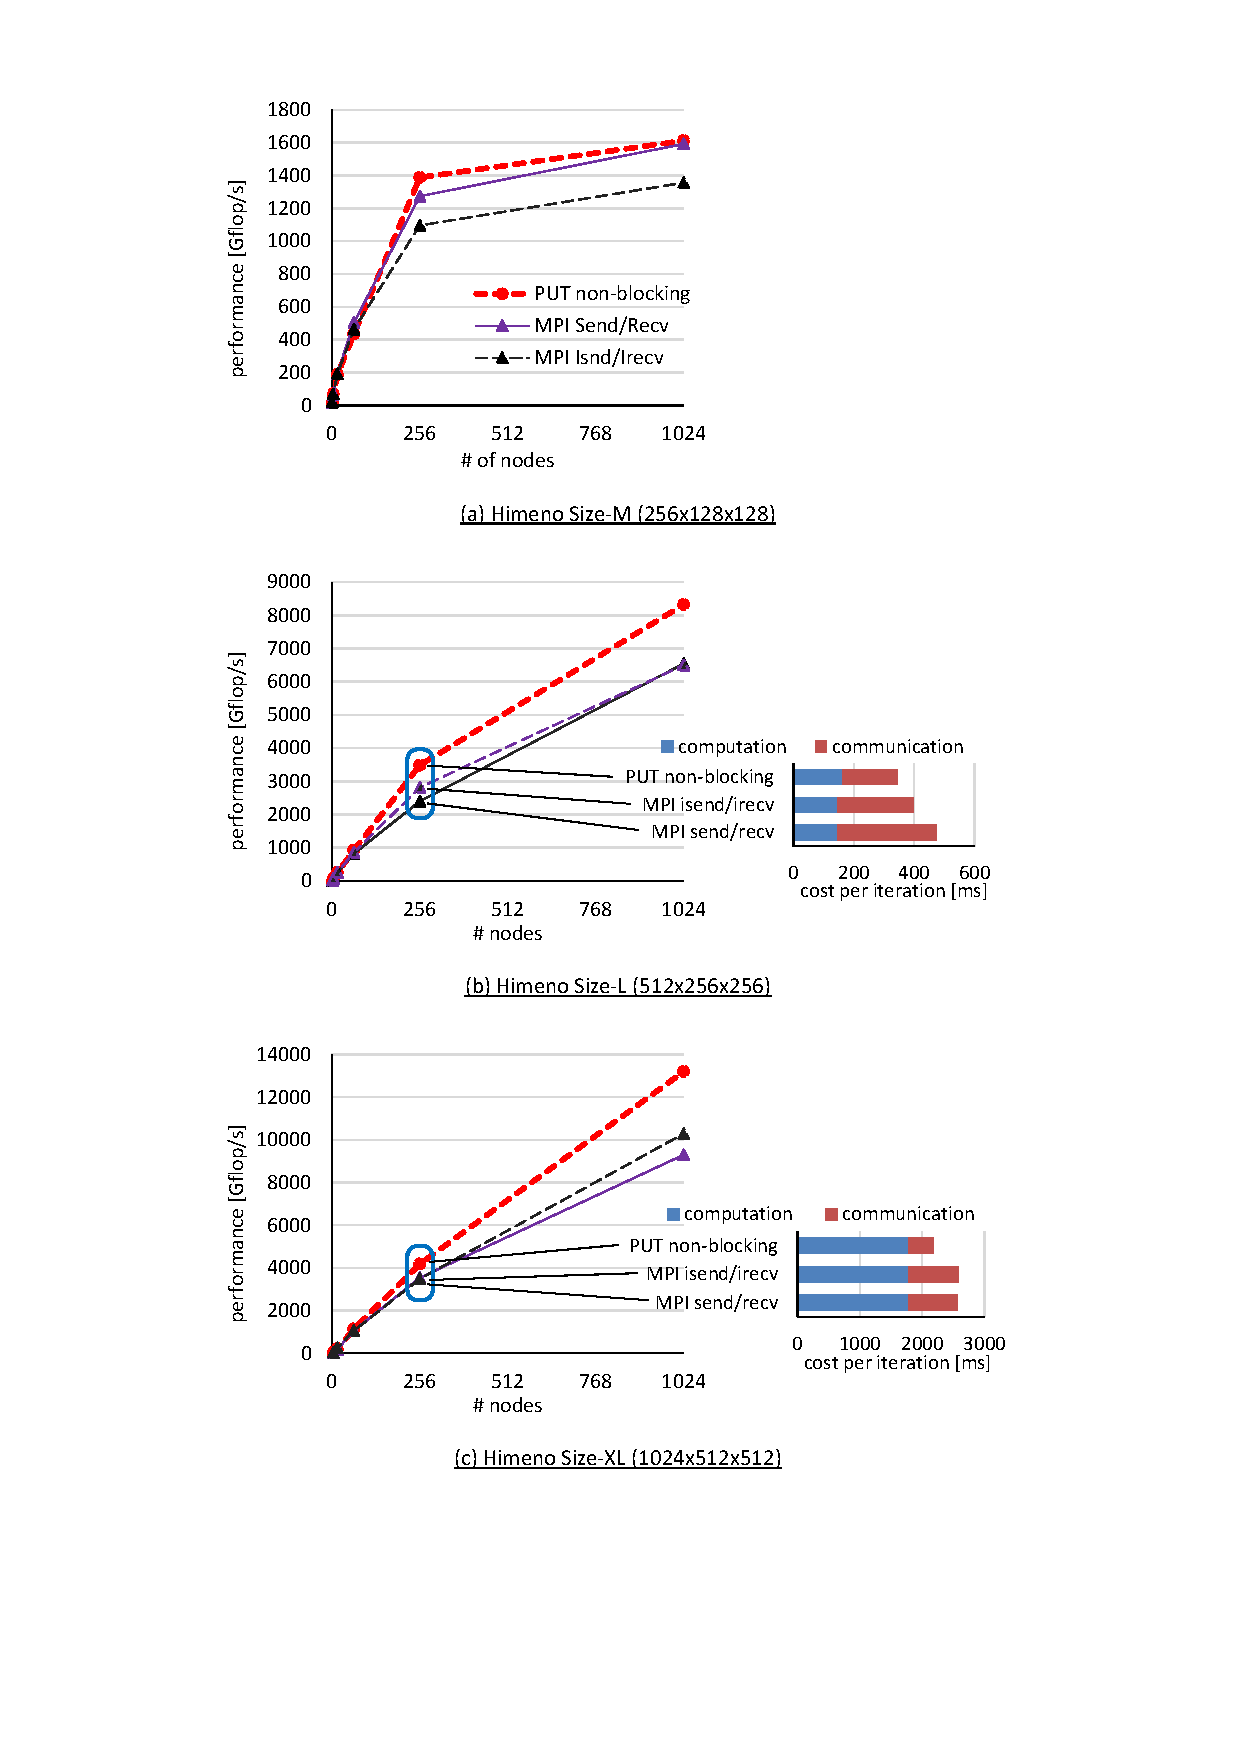
\includegraphics[trim=37mm 34mm 37mm 4mm, scale=0.8,clip]{figs/himeno-graph-r2.pdf}}
    \caption{himeno-graph-r2.pdf}\label{fig:himeno-graph}
  \end{center}
\end{figure}


マシン名要確認。ころころ変えていないか。


% %-- 3cell-y.pdf
% %-- 3cell-z.pdf
% \begin{figure}[tbh]
%   \begin{center}
%   % trimはleft bottom right topの順
%   \fbox{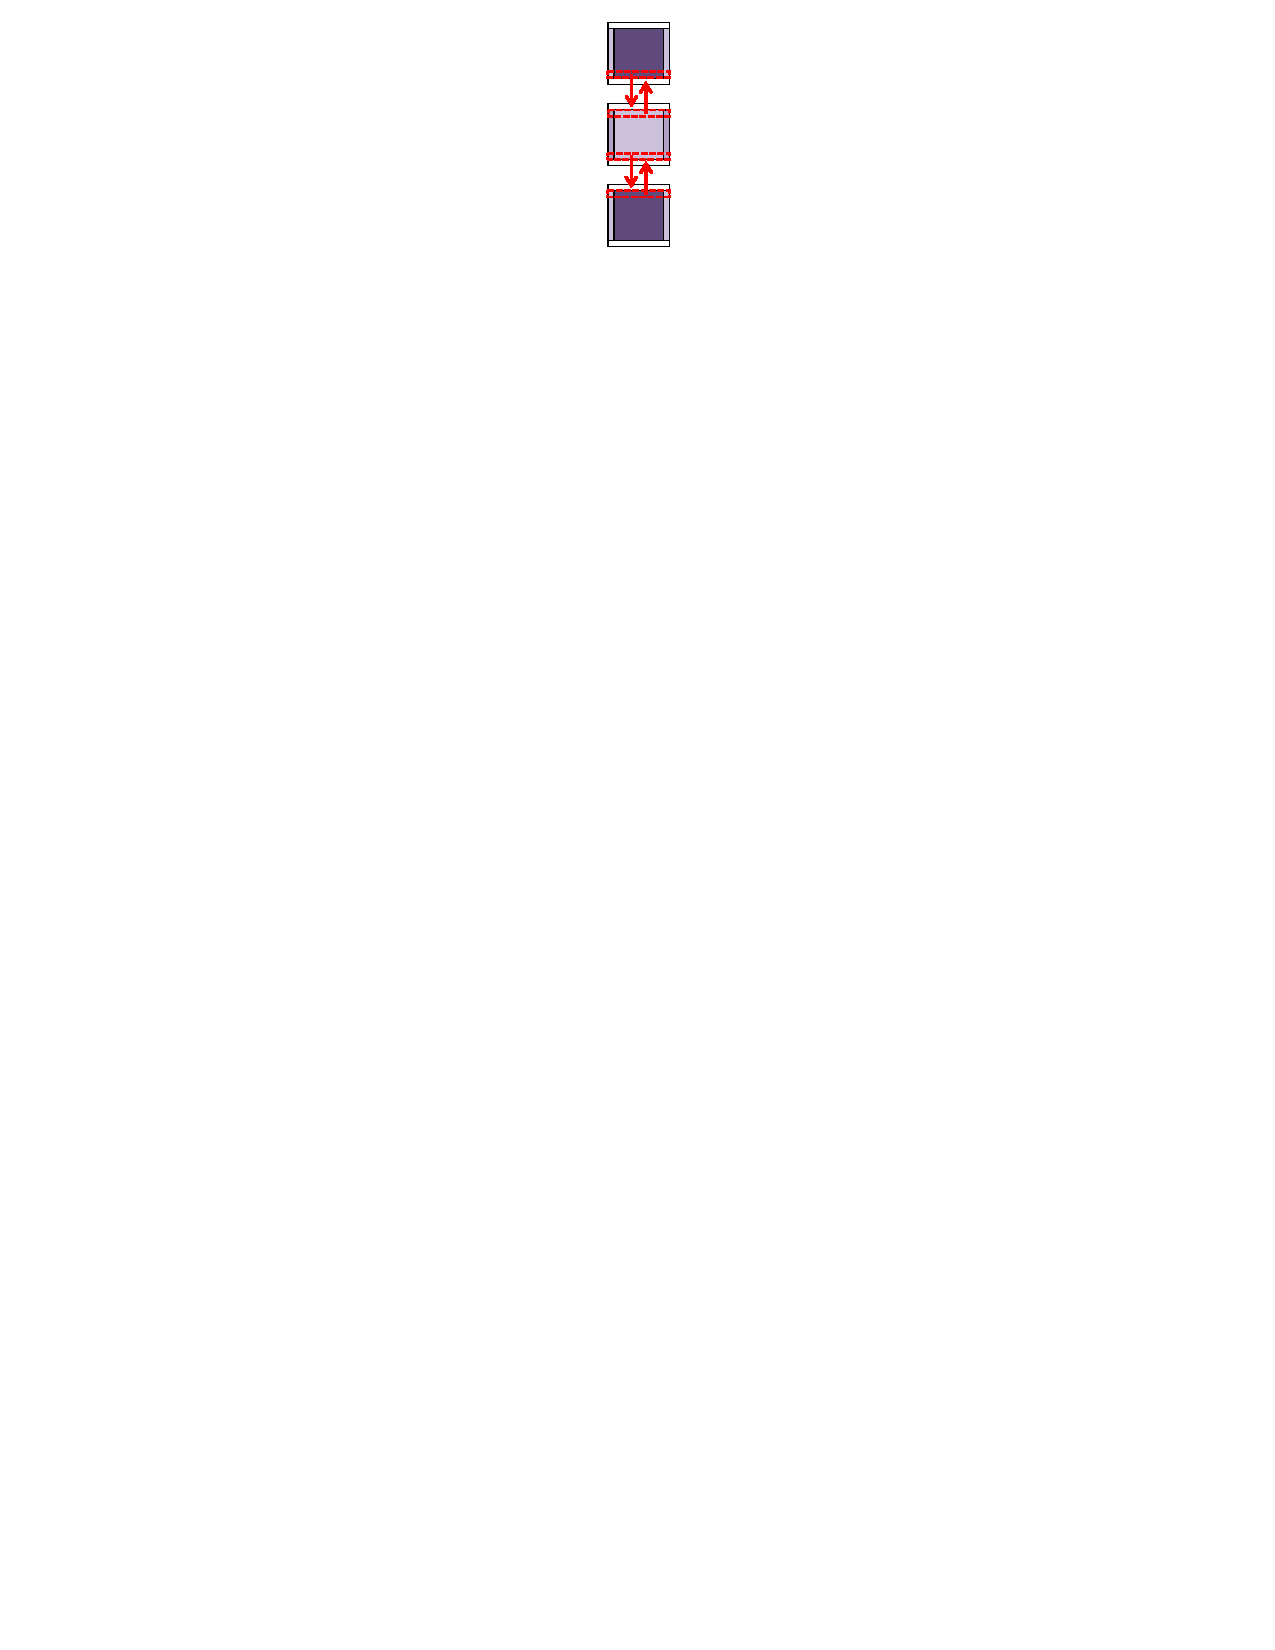
\includegraphics[trim=98mm 235mm 98mm 0mm, scale=0.8,clip]{figs/3cell-y.pdf}}  \\
%   \fbox{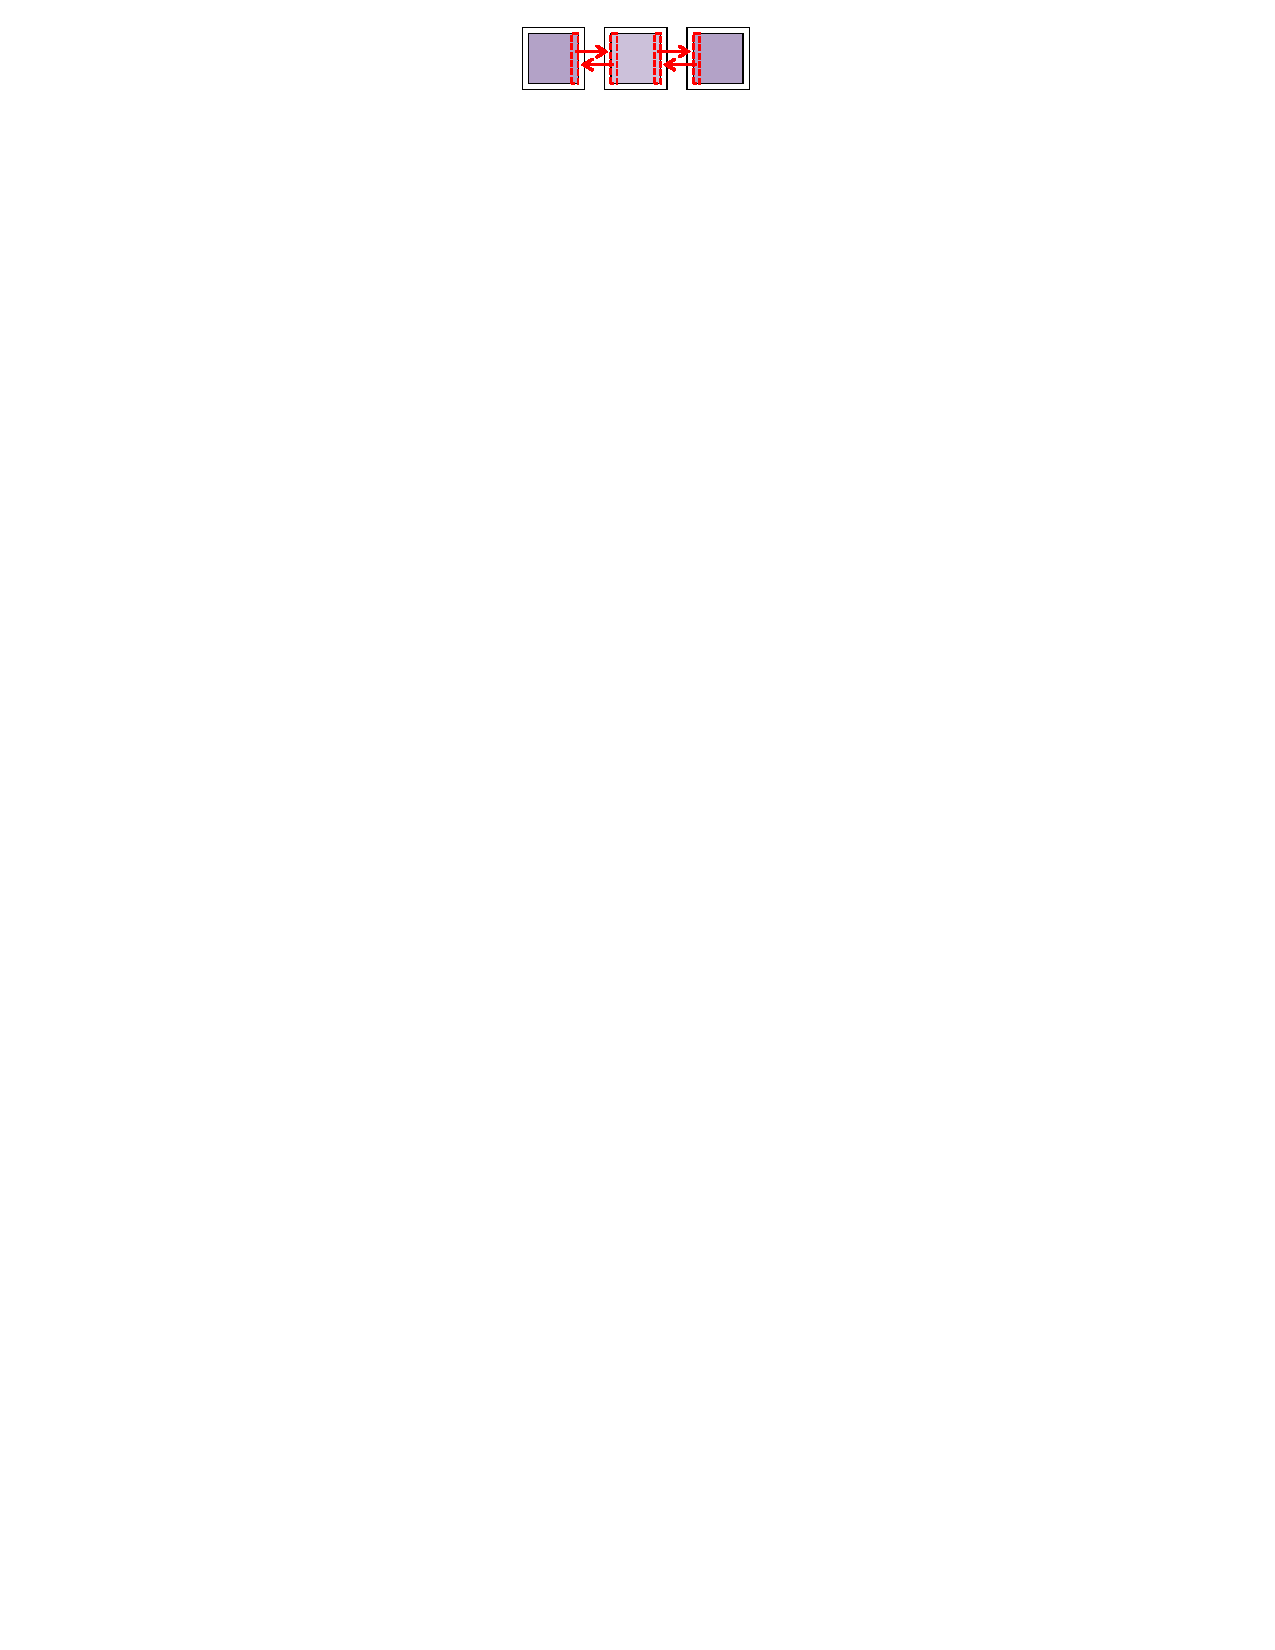
\includegraphics[trim=85mm 261mm 85mm 0mm, scale=0.8,clip]{figs/3cell-z.pdf}}  \\
%   \fbox{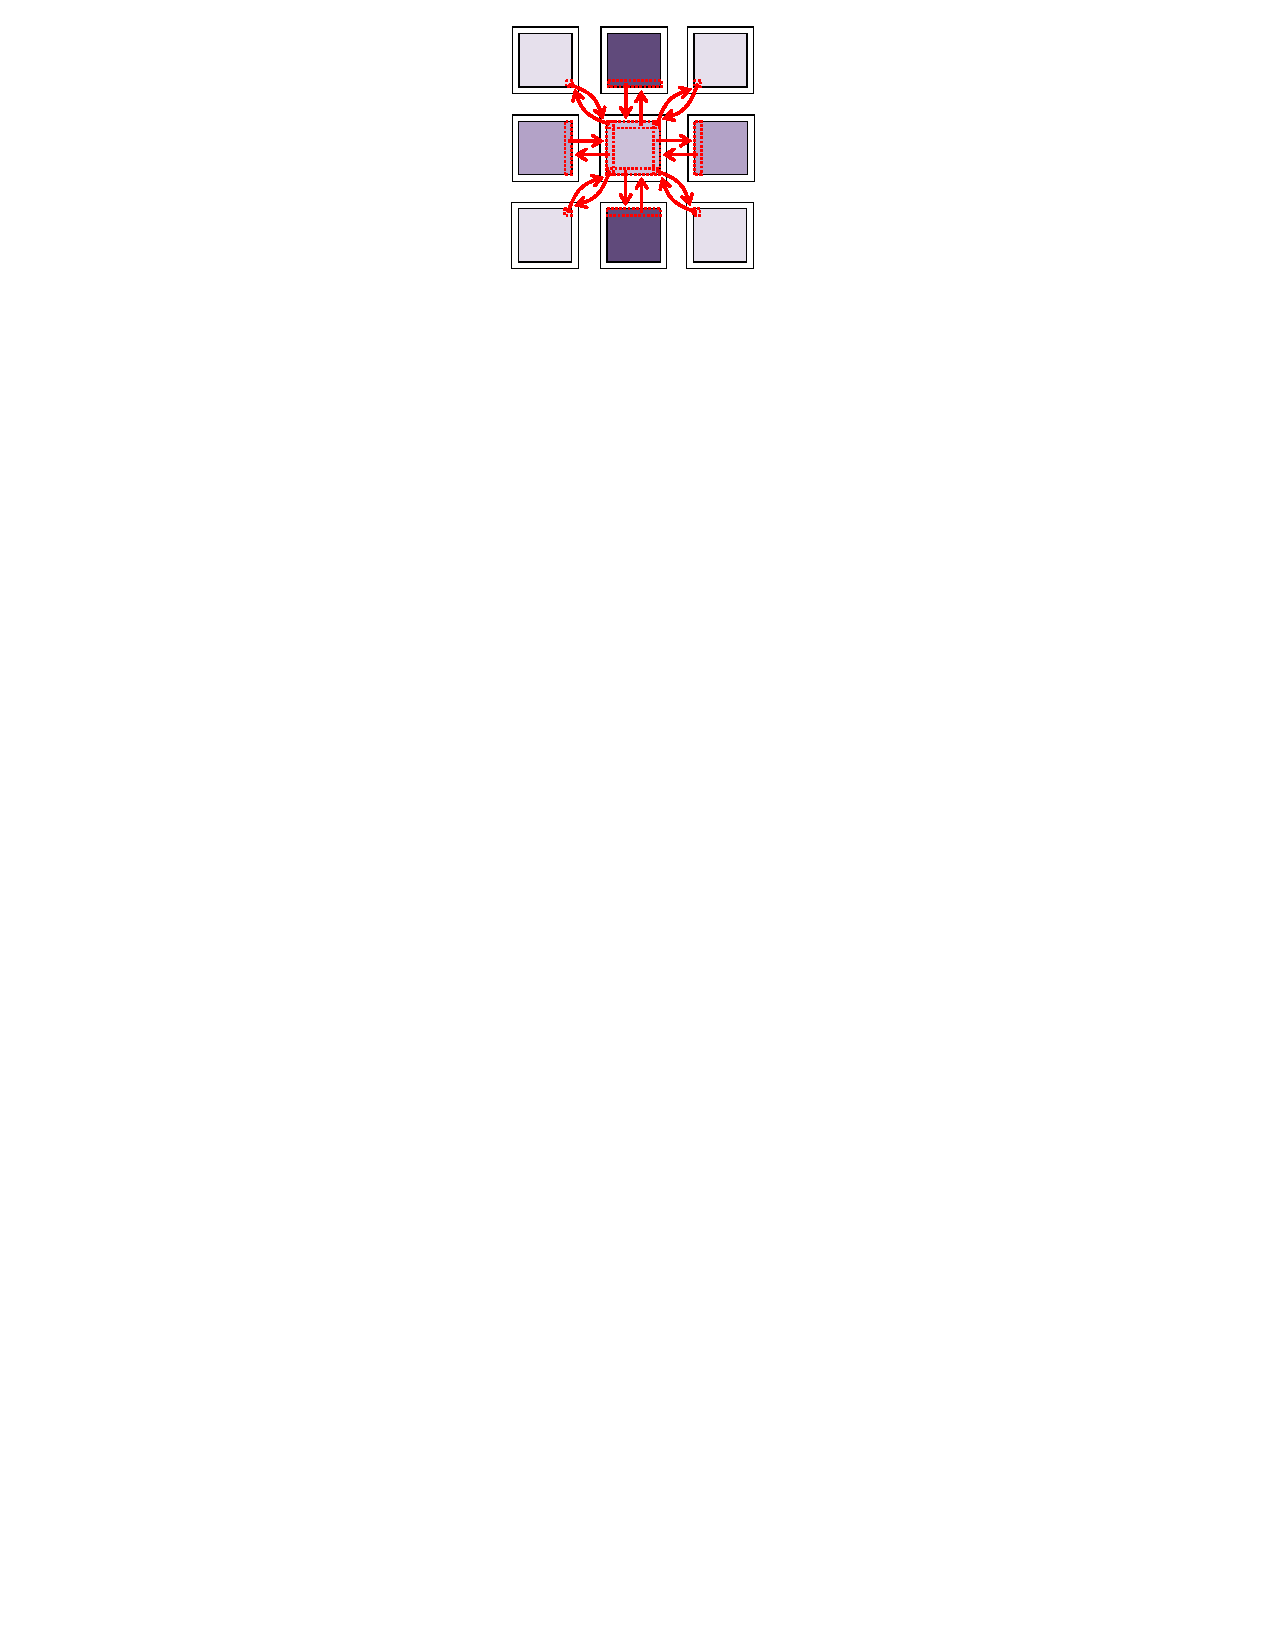
\includegraphics[trim=82mm 230mm 84mm 0mm, scale=0.8,clip]{figs/9cell-yz.pdf}}
%   \caption{3cell-y.pdf, 3cell-z.pdf, 9cell-yz.pdf}\label{fig:cell}
%   \end{center}
% \end{figure}


%-- fx100-pipo.pdf
%    \fbox{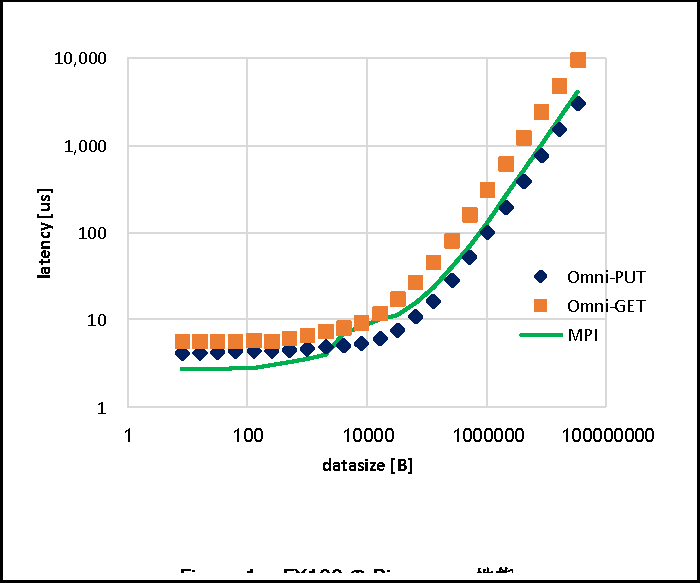
\includegraphics[trim=4mm 15mm 4mm 3mm, scale=0.9,clip]{figs/fx100-pipo.pdf}}

%himeno.pdf
%latency-16var.pdf
%layer.pdf

%register-CA-tmp.pdf
%register-RA-CA-tmp.pdf
%register-RA-tmp.pdf
%softstack.pdf
%translator-tmp.pdf
